\documentclass[a4paper,12pt]{article}
\usepackage{fancyhdr}
\usepackage{fancyheadings}
\usepackage[ngerman,german]{babel}
\usepackage{german}
%\usepackage[latin1]{inputenc}
\usepackage[active]{srcltx}
\usepackage{algorithm}
\usepackage[noend]{algorithmic}
\usepackage{amsmath}
\usepackage{amssymb}
\usepackage{amsthm}
\usepackage{bbm}
\usepackage{enumerate}
\usepackage{graphicx}
\usepackage{ifthen}
\usepackage{listings}
\usepackage{struktex}
\usepackage{hyperref}
\usepackage[breakable]{tcolorbox}
\usepackage[a4paper, left=2cm, right=2cm, top=2cm]{geometry}
\usepackage{mathtools}
\usepackage{tikz}
\usepackage{dsfont}
\usepackage{multicol}
\usepackage{pgfplots}
\usepackage{comment}
\usepackage{systeme}
\usepackage{gauss}
\usepackage{wrapfig}

\usetikzlibrary{3d}
\syscodeextracol{\quad\hfill}{\hfill}
\sysautonum*{(\uppercase\expandafter{\romannumeral*})}
\sysdelim..
\usetikzlibrary{trees}
\pgfplotsset{compat=newest}

\tikzstyle{level 1}=[level distance=3.5cm, sibling distance=4.5cm]
\tikzstyle{level 2}=[level distance=3.5cm, sibling distance=2cm]



% Define styles for bags and leafs
\tikzstyle{bag} = [text width=2em, text centered]
\tikzstyle{end} = [circle, minimum width=3pt,fill, inner sep=1pt]

\newcommand{\contradiction}{{\hbox{%
			\setbox0=\hbox{$\mkern-3mu\times\mkern-3mu$}%
			\setbox1=\hbox to0pt{\hss$\times$\hss}%
			\copy0\raisebox{0.5\wd0}{\copy1}\raisebox{-0.5\wd0}{\box1}\box0
}}}
\definecolor{dg}{HTML}{00997b}
\definecolor{lightblue}{HTML}{8920ff}
\definecolor{darkblue}{HTML}{000099}
\definecolor{lightred}{HTML}{ff2089}
\definecolor{darkred}{HTML}{990000}
%%%%%%%%%%%%%%%%%%%%%%%%%%%%%%%%%%%%%%%%%%%%%%%%%%%%%%
\newcommand{\Fach}{Grenzwerte}
\newcommand{\Semester}{SoSe 21}
\newcommand{\Uebungsblatt}{Analytische Geometrie} 
\newcommand{\nl}{\\[0,20cm]}
\newcommand{\lnl}{\\[0,30cm]}
\newcommand{\xlnl}{\\[0,75cm]}
%%%%%%%%%%%%%%%%%%%%%%%%%%%%%%%%%%%%%%%%%%%%%%%%%%%%%%


\setlength{\parindent}{0em}
\topmargin -2.0cm
\oddsidemargin 0cm
\evensidemargin 0cm
\setlength{\textheight}{9.6in}
\setlength{\textwidth}{5.9in}
\addtolength{\hoffset}{16pt}


\newcommand{\limes}[2]{
	\lim\limits_{x\rightarrow #1}\quad  #2
}
\newcommand{\limesh}[1]{
	\lim\limits_{h\rightarrow 0}\quad  #1
}
\newcommand{\limesr}[2]{
	\lim\limits_{\underset{x > #1}{x\rightarrow #1}}\quad  #2
}
\newcommand{\limesl}[2]{
	\lim\limits_{\underset{x < #1}{x\rightarrow #1}}\quad  #2
}
\newcommand{\Redbox}[1]{
	{
		\vspace*{0.1cm}
		\begin{tcolorbox}[breakable,colback=yellow!0,colframe=red!65!black,width=\linewidth ]
			{#1}
		\end{tcolorbox}
		
		
	}
}
\newcommand{\Aufgabe}[2]{
	{
		\vspace*{0.3cm}
		\begin{tcolorbox}[breakable,colback=yellow!0,colframe=black!65!white,title=\textbf{Aufgabe #1:},width=\linewidth ]
			{#2}
		\end{tcolorbox}
		
		
	}
}
\newcommand{\Definition}[2]{
	{
		\vspace*{0.1cm}
		\begin{tcolorbox}[breakable,colback=yellow!0,colframe=black!40!red,title=\textbf{Definition #1:},width=\linewidth ]
			{#2}
		\end{tcolorbox}
		
		
	}
}
\newcommand{\Hinweis}[1]{
	\vspace*{0.3cm}
	\begin{tcolorbox}[breakable,colback=yellow!10,colframe=yellow!65!black,title=\textbf{Hinweis:},width=\linewidth ]
		{#1}
	\end{tcolorbox}
}
\newcommand{\SHA}[1]{
	\vspace*{0.1cm}
	\begin{tcolorbox}[breakable,colback=blue!5,colframe=blue!65!black,title=\textbf{Richtiger SHA256 Hash:},width=\linewidth ]
		{\texttt{{#1}}}
	\end{tcolorbox}
}
\newcommand{\Beispiel}[1]{
	\vspace*{0.2cm}
	\begin{tcolorbox}[breakable,colback=yellow!0,colframe=green!65!black,title=\textbf{Beispiel:},width=\linewidth ]
		{#1}
	\end{tcolorbox}
}
\newcommand{\p}[2]{\pi_{#2}^{(#1)}}
\newcommand{\eing}[1]{\begin{enumerate}[\quad]
		\item #1
\end{enumerate}}

\newcommand{\abc}[1]{
	\begin{enumerate}[(a)]
		#1
	\end{enumerate}
}
\makeatletter
\newcommand{\Spvek}[2][r]{%
	\gdef\@VORNE{1}
	\left(\hskip-\arraycolsep%
	\begin{array}{#1}\vekSp@lten{#2}\end{array}%
	\hskip-\arraycolsep\right)}

\def\vekSp@lten#1{\xvekSp@lten#1;vekL@stLine;}
\def\vekL@stLine{vekL@stLine}
\def\xvekSp@lten#1;{\def\temp{#1}%
	\ifx\temp\vekL@stLine
	\else
	\ifnum\@VORNE=1\gdef\@VORNE{0}
	\else\@arraycr\fi%
	#1%
	\expandafter\xvekSp@lten
	\fi}
\makeatother
\newcommand{\integral}[4]{\int\limits_{#1}^{#2} {#3} {\quad d #4}}
\newcommand{\summe}[3]{\sum\limits_{#1}^{#2} #3}
\begin{document}
	\pagestyle{fancy}
	\begin{center}
		\LARGE \sf \textbf{ \Uebungsblatt{}}
	\end{center}
	
	\vspace*{0.1cm}
	
		
	
	\section{Einführung}
	Viele Anwendungsfälle der Mathematik in der heutigen Welt sind geometrische Rechnungen im Mehrdimensionalen Raum. So werde diese in verschiedener Planungssoftware zur Konstruktion von so gut wie allen Dingen heutzutage eingesetzt. Für die Brückenplanung nutzt der Bauingeneur Auto-CAD, zum Planen der neuen Küche manche den IKEA-Küchenplaner und Vectary zum Planen von Drucken für den 3D-Drucker.\\
	Die bisher gelernten Beschreibungsarten für Geometrie sind leider bisher noch nicht so mächtig wie wir sie gerne hätten. So versuche zum Beispiel Eine Gerade im 2 dimensionalen Raum, welche parallel zur y-Achse ist, zu beschreiben. Dies ist mit dem herkömmlichen $y=mx+n$ unmöglich. Gleichzeitig wollen wir nicht nur im 2-Dimensionalen, sondern auch $n$-Dimensionalen Raum arbeiten und dort zum Beispiel den Abstand von 2 diskreten Punken oder Objekten berechnen.\\ 
	\section{Lineare Gleichungssysteme}
	Lineare Gleichungssysteme sind eines der meißtgenutzten Konzepte der Mathematik. Diese sind Teil der Lösungen verschiedener Probleme in der Mathematik und auch echten Welt. So zum Beispiel in Viedospielen, Computertomographie elektrische Spannungen in vermaschten Stromkreisen und das erstellen von CPU-Architekturen. Est ist eine einfache mathematische Version dessen was man im Allgemeinen als Deduktion bezeichnet. Dabei wird aus einer Grundmenge von Information neue Information hergeleite, welche mit der gegebenen konsistent ist, d.h. sich nicht gegenseitig ausschließt.\\\\
	Lineare Gleichungssysteme bestehen dabei aus $N$ Zeilen. Wir nennen diese meist $I,II,III,IV,...\,$. Jede Zeile ist dabei eine Gleichung mit $n$ linearen Variablen. Linear heißt dabei: keine Variable hat einen Exponenten ungleich 1.
		\Redbox{\begin{align*}
				k_{1;1}\cdot x_1 + k_{1;2}\cdot x_2+ ... + k_{1;n}\cdot x_n 	&=d_1&&\text{(I)}\\
				k_{2;1}\cdot x_1 + k_{2;2}\cdot x_2+ ... + k_{2;n}\cdot x_n 	&=d_2&&\text{(II)}\\
				k_{3;1}\cdot x_1 + k_{3;2}\cdot x_2+ ... + k_{3;n}\cdot x_n 	&=d_3&&\text{(III)}\\
				\vdots\qquad \qquad\qquad  &\vdots &&\,\,\vdots\\
				k_{N;1}\cdot x_1 + k_{N;2}\cdot x_2+ ... + k_{N;n}\cdot x_n 	&=d_N&&\text{(N)}\\\\
				\text{mit } d_j,\,k_{j;i}\in \mathds{R},\text{ für } i=1,...,n,\quad j=1,...,N &\text{ und } x_1,...,x_n \text{ Variablen} 
		\end{align*}}
	Dabei steht $j$ für die Zeilennummer und $i$ für die Nummer der zugehörigen Variable. Ein kleines Beispiel zeigt dies etwas übersichtlicher:
	\[\systeme{
		3x_1 + 2x_2 - x_3 = 1,
		2x_1 - 2x_2 + 4x_3 = -2,
		-x_1 + \frac{1}{2}x_2 - x_3 = 0
	}\]
	Für bessere Übersichtlichkeit werden in den Aufgaben Variablen $w,x,y,z$ verwendet werden, statt $x_1,x_2,x_3,x_4$.\\
	Natürlich können solche Gleichungssysteme auch ander aussehen, lassen sich aber immer in diese Form transformieren.
	\subsection{Vorbetrachtungen}
	Wie bei allem in Mathe sollte man bevor man sich in die Rechenarbeit stürzt ein paar Vorüberlegungen zur Aufgabe machen um potentiell Rechenarbeit zu sparen und schon eine ''Idee'' vom Ergebnis zu haben.\\
	Das Wichtigste dabei ist der Vergleich zwischen Anzahl der Variablen $n$ und Anzahl der Gleichungen $N$. Dabei gilt:
	\Redbox{\begin{itemize}
			\item für $N<n$ gibt es definitiv keine eindeutige Lösung. Die Lösungsmenge $\mathds{L}$ ist unendlich groß und, das sei hier nur am Rande erwähnt, größer gleich $ N-n$ dimensional.
			\item für $N\geq n$ kann es eine eindeutige Lösung geben, muss es aber nicht. Dies hängt davon ab, ob die Gleichungen linear unabhängig voneinander sind. Was das genau heißt ist hier nicht so wichtig, interessierte können dafür jedoch gerne mal im Internet stöbern oder darüber meditieren. \\
			Im Fall $N > n$ kann es auch eine leere Lösungsmenge geben $\mathds{L}=\emptyset$, dann gibt es keine ''richtige'' Wahl der Variablen, also eine Wahl mit welcher alle Gleichungen wahr werden. 
	\end{itemize}}
	Nach dieser kleinen Vorbetrachtung schauen wir uns 4 verschiedene Arten an solche Gleichungssysteme zu lösen, dabei sollten die ersten Beiden bereits bekannt sein. Jedes Verfahren hat natürlich seine Vor- und Nachteile, aus meinser Sicht ist das Gauss-Jordan Verfahren der beste Allrounder, gerade für große Gleichungssysteme.
	\subsection{Einsetzungsverfahren}
	Das Einsetzungsverfahren ist relativ simpel. Es eignet sich hierbei gerade wenn das, am besten kleine, Gleichungssystem noch nicht richtig umgestellt wurde. \\
	Dabei wird eine der Gleichungen nach einer Variable umgestellt. In eine andere Gleichung des Gleichungssystems kann man nun diese Variable ersetzen.
	\Beispiel{\[\systeme{
			9x-y=41,
			3x-11=y
		}\]
		Einsetzen von (II) in (I):
		\begin{align*}
			9x- (3x-11)&=41&&\\
			9x- 3x+11&=41&&|-11\\
			6x&=30&&|:6\\
			x&=5&&\text{Lösung in (II) einsetzen}\\
			y&=3\cdot 5 - 11 =4\\\\
			\implies \mathds{L}&=\{(5\,|\,4)\}
		\end{align*}
	}
	Ich empfehle dieses Verfahren nur bei Gleichungssystem mit 2 Gleichungen zu nutzen, oder es mit einem der anderen zu paaren.
	\Aufgabe{2.2.1: (Finde die Lösungsmenge mittels Einsetzungsverfahren)}{
		\begin{multicols}{2}
			\begin{enumerate}[(a)]
				\item $\systeme{3x+4=y,
					4y-3x=9}$
				\item $\systeme{x - 3y + 5z = -2,
					y + 2z = 8,
					y + z =6}$
				\item $\systeme{x + 4y - z = 13,
					3y + 2z = 21,
					3z = 9}$
				\item $\systeme{3x - 2y + 2z = 6,
					2x - z = 2,
					-3x = -6}$
			\end{enumerate}
		\end{multicols}
	}
	\subsection{Gleichsetzungsverfahren}
	Eine zum Einsetzungsverfahren ähnliche Methode. Hierbei wählt man 2 Gleichungen des Gleichungssystems aus, wobei diese eine Seite des ''$=$'' gemeinsam haben müssen, also dort steht das Gleiche. Dadurch können wir diese Gleichungen gleichsetzen. Oft muss man mindestens eine Gleichung umstellen um diese Ausgangssituation zu bekommen.
	\Beispiel{
		\[\systeme{
			3x + 6y = 9,
			5 + 3y = \color{red}x\color{black}
		}\]
		Umstellen von (I) nach $x$
		\begin{align*}
			\rightarrow \quad \color{red}x\color{black}&=3-2y\\
			\text{ Gleichsetzen }(\color{red}x\color{black}):&\\
			5 + 3y &= 3-2y &&| +2y,\, -5\\
			5y &= -2 &&| :5\\
			y&=-\frac{2}{5}\\
			\text{Ergebnis in (II) einsetzen}\\
			x&=5+3y=5+3\cdot (-\frac{2}{5})=\frac{25}{5} - \frac{6}{5}= \frac{19}{5}\\\\
			\implies \quad\mathds{L}&=\left\{\left(\frac{19}{5}\,\,\bigg\vert \, -\frac{2}{5}\right) \right\}
		\end{align*}
	}
	Wie auch das vorherige Verfahren empfehle ich dieses eher bei kleinen Gleichungssystemen und wo sich das Gleichsetzen auch anbietet, also nicht zu viel umzustellen ist. 
	  \Aufgabe{2.3.1: (Finde die Lösungsmenge mittels Gleichsetzungsverfahren)}{
		\begin{multicols}{2}
			\begin{enumerate}[(a)]
				\item $\systeme{y=4x+6,
					y=-2x+3}$
				\item $\systeme{3y=2x-7,
					3y=x-3}$
			\end{enumerate}
		\end{multicols}
	}
	\subsection{Additionsverfahren}
	Ein Verfahren auch für größere Gleichungssysteme geeignet ist das Additionsverfahren. Dabei werden ganze Gleichungen (Zeilen) miteinander addiert und subtrahiert, um eine bestimmte Variable zu eliminieren. Dabei können die Zeilen vor diesem schritt mit einem Koeffizienten multipliziert werden damit sicher eine Variable eliminiert werden kann. Eine solche Addition oder Subtraktion läuft dabei Komponentweise ab, d.h. werden die Koeffizienten, zugehörig zur gleichen Variable, miteinander addiert oder subtrahiert.
	\Redbox{
		\begin{align*}
				k_{i;1}\cdot x_1 + k_{i;2}\cdot x_2+ ... + k_{i;n}\cdot x_n 	&=d_i&&\text{(i)}\\
				k_{j;1}\cdot x_1 + k_{j;2}\cdot x_2+ ... + k_{j;n}\cdot x_n 	&=d_j&&\text{(j)}\\
				&\downarrow\\
				(r k_{j;1} + t k_{i;1})\cdot x_1 +  ... + (r k_{j;n} + tk_{i;n})\cdot x_n 	&=r d_j + td_i &&r\text{(j)} +t\text{(i)}\\
				\text{Um Variable }x_1\text{ zu eliminieren wählen wir } &r,t\text{ so}:\\
				r=\frac{kgV(k_{i;1},k_{j;1})}{k_{j;1}}\quad & \quad t=-\frac{kgV(k_{i;1},k_{j;1})}{k_{i;1}}
		\end{align*}
	}
Dadurch werden $r,t$ so gewählt das der Koeffizient von $x_1$ 0 ergibt. Und $kgV$ steht hierbei für das kleinste gemeinsame Vielfache der beiden Zahlen.\\
\Beispiel{
	\[\systeme{
		\color{blue}2\color{black}x + 3y = 14,
		\color{blue}1\color{black}x + 2y = 8
	}\]
	Wir wollen $x$ eliminieren und da  $2 \cdot \color{blue}1\color{black} = \color{blue}2\color{black}$ müssen wir rechnen (I) $- 2\cdot $(II)
	\begin{align*}
		\rightarrow\qquad  - 2x - 4y &= -16 &&| -2\cdot \text{(II)}\\\\
		\text{(I)} - 2\cdot\text{(II)}:\qquad \qquad (2-2)x + (3-4)y&= (14 - 16)\\
		0x - 1y = -2\\
													-y&=-2 \quad\implies\quad y=2\\
													\text{ Ergebnis in (II) einsetzen}&\\
													x+ 2\cdot(-2)&=8&&|+4\\
													x&=12\\\\
													\implies \quad \mathds{L}&=\{(12\,|\,-2)\}												 
	\end{align*}
	}
	Dieses Verfahren ist gut geeignet zum Lösen von großen Gleichungssystemen, da es übersichtlich bleibt. Da man sich aussuchen kann welche Variable eliminiert wird kann, bei cleverer herangehensweise selbst große systeme sehr schnell gelöst werden.\\
	Eine Veralgemeinerung des Verfahrens genannt Gauss Algorithmus nutzt eben dieses verfahren um mit einer festen Handlungsabfolge solche Gleichungssysteme $N=m$ zu lösen.
	\subsection{Gauss-Algorithmus}
	Der Gauß Algorithmus nutzt das Additionsverfahren und setzt dies ein um strukturiert die Variablen nacheinander zu eliminieren. Im ersten Schritt werden die $x$-Variablen mit Hilfe der ersten Gleichung aus den anderen Gleichungen eliminiert. Anschließend wird die $y$-Variable mit Hilfe der zweiten Gleichung aus den darunterliegenden Gleichungen eliminiert usw..
	\Beispiel{
		\[\systeme{
			x+y+2z=12,
			3x-2y-5z=7,
			x+2y-z=-3
		}\]
		mit (II) $-\,3\cdot$(I) und (III) $-$ (I) 
		\[\systeme{
			x+y+2z=12,
			-5y-11z=-29,
			y-3z=-15
		}\]
		vertauschen der Zeile (II) und (III)
		\[\systeme{
			x+y+2z=12,
			y-3z=-15,
			-5y-11z=-29
		}\]
		(III) $+\, 5\cdot $(II)
		\[\systeme{
			x+y+2z=12,
			y-3z=-15,
			-26z=-104
		}\]
	\begin{align*}
		\implies \quad z&=\frac{-104}{-26}=\frac{104}{26}=4\\\\
		y-3z&=-15&&| \,Einsetzen\\
		y-3\cdot 4&=-15		&& | +12\\
		y&=-3\\\\
		x+y+2z&=12 &&|\, Einsetzen\\
		x-3+2\cdot 4&=12&&| -5\\
		x&=7\\\\
		\implies \mathds{L}=\{(7\,|\,-3\,|\,4)\}
	\end{align*}
	}
Ein kleiner Hinweis zur Notation: Um sich Schreibarbeit zu sparen kann man die Variablen weglassen und lediglich die Zahlen schreiben. Es folgt das selbe Beispiel in anderer Notation.
	\Beispiel{
		\begin{align*}
			&\begin{gmatrix}[v]
				1 & 1 & 2 & 12 \\
				3 & -2 & -5 & 7 \\
				1 & 2 & -1 & -3
				\rowops
				\add[-3\cdot\,]{0}{1}
				\add[-1\cdot]{0}{2}
				\swap{1}{2}
			\end{gmatrix}\\\\
	&\begin{gmatrix}[v]
		1 & 1 & 2 & 12 \\
		0 & 1 & -3 & -15\\
		0 & -5 & -11 & -29		
		\rowops
		\add[5\cdot]{1}{2}
	\end{gmatrix}\\\\
&\begin{gmatrix}[v]
	1 & 1 & 2 & 12 \\
	0 & 1 & -3 & -15\\
	0 & 0 & -26 & -104		
\end{gmatrix}\\\\
\implies \quad z&=\frac{-104}{-26}=\frac{104}{26}=4\\\\
y-3z&=-15&&| \,Einsetzen\\
y-3\cdot 4&=-15		&& | +12\\
y&=-3\\\\
x+y+2z&=12 &&|\, Einsetzen\\
x-3+2\cdot 4&=12&&| -5\\
x&=7\\\\
\implies \mathds{L}=\{(7\,|\,-3\,|\,4)\}
		\end{align*}
	
	}
	


\Aufgabe{2.6.2 (Finde die Lösungsmenge mittels Gauss-Verfahren)}{
		\begin{multicols}{2}
			\begin{enumerate}[(a)]
				\item $\systeme{2x + 3y - 2z = 0,
					y + z = -1,
					-x + 2y + 3z = -5}$
				\item $\systeme{x - y + 2z = 0,
								-2x + y -6z = 0,
								x - 2z = 3}$
				\item $\systeme{ 4x + 9y + 5z = 13,
					-5x + 6y + 3z = 17,
					6x + 3y - 10z = 23}$
				\item $\systeme{2a + 3b - c + 5d = 11,
								 b + 3c - d = 1,
							 	4a - 2b- 2d = 0,
						 		 a + b + c + d =4}$
				\item $\systeme{\frac{1}{4}x -\frac{1}{2}y + \frac{3}{4}z = 4,
				\frac{3}{2}x - \frac{2}{3}y - \frac{1}{2}z = -2,
				y - \frac{1}{2}z=2}$
			\end{enumerate}
		\end{multicols}
	}

\Aufgabe{2.6.3 (Untersuche auf Lösbarkeit und gib die Lösungsmenge an)}{
	\begin{multicols}{2}
		\begin{enumerate}[(a)]
			\item $\systeme{ 2x + 2y + 2z = 6,
							2x + y - z = 2,
							4x + 3y + z = 8}$
			\item $\systeme{3x + 5y - 2z = 10,
							2x + 8y - 5z = 6,
							4x + 2y + z = 8}$
		\end{enumerate}
	\end{multicols}
}
\Aufgabe{2.6.4 (Löse die Textaufgaben mittels Gleichungssystem)}{
	\begin{multicols}{2}
		\begin{enumerate}[(a)]
			\item Fünf Ochsen und zwei Schafe kosten acht Goldstücke, zwei Ochsen und acht Schafe kosten acht Goldstücke. Wie hoch ist der Preis für jedes einzelne Tier?
			\item In einem Käfig sind Hasen und Fasane. Sie haben zusammen 35 Köpfe und 94 Füße. Wie viele Hasen und Fasane sind im Käfig?
			\item In einem Jugendheim gibt es 18 Zimmer (Vierbett- und Sechsbettzimmer). Insgesamt können 84 Jugendliche untergebracht werden. Wie viele Vierbett- bzw. Sechsbettzimmer	sind es?
			\item Zwei Tassen Kaffee und ein Stück Kuchen kosten 8,00 \$, drei Tassen Kaffee und vier Stück Kuchen kosten 20,00 \$. Berechnen Sie den Preis für eine Tasse Kaffee bzw. ein	Stück Kuchen.
		\end{enumerate}
	\end{multicols}
}
\newpage
	\section{Vektorarithmetik}
	Bevor wir wieder zu Gleichungssystemen kommen müssen wir über ein neu einzuführendes Konzept reden. Dies ist ähnlich gegenüber dem ist was wir als Punkt kennen. Nach Pythagoras: ''\textit{Ein Punkt ist als Einheit (monas), die eine Position hat, zu verstehen.}'' Die Einheit besitzt dabei keine Ausdehnung (Volumen).\\
	Wenn wir nun von einem fest gewähltem Punkt $U$ aus einen anderen Punkt $P$ betrachten, können wir $P$ auch beschreiben durch die Richtung und Entfernung die wir von $U$ aus gehen müssen um zu $P$ zu kommen. 
	\subsection{Vektoren}
	\Definition{(Vektor)}{
		Ein Vektor, geschrieben $\vec{v}$, wird beschrieben durch eine Richtung in die er zeigt und einer Länge. Man kann sich Vektoren bildlich wie Pfeile vorstellen. Die eigentliche Interpretation ist eine Verschiebung im Raum.
		\begin{center}
			\begin{tikzpicture}
				\draw[thin,gray!40] (-2,-2) grid (4,4);
				\draw (-1,0) node[anchor=south] {$U$};
				\draw (-1,0) node {$\times$};
				\draw (3,3) node[anchor=south] {$P$};
				\draw (3,3) node {$\times$};
				\draw[line width=2pt,blue,-stealth](-1,0)--node[anchor=north west]{$\vec{v}$} (3,3) ;
				\draw (3,-1) node[anchor=south] {$T$};
				\draw (3,-1) node {$\times$};
				\draw[line width=2pt,red,-stealth](-1,0)--node[anchor=north west]{$\vec{u}$} (3,-1) ;
			\end{tikzpicture}\\
		\end{center}
			Je nachdem in wie vielen Dimensionen wir uns bewegen, oben 2 Dimensionen, werden Vektoren anders angegeben. \\
	Ein Vektor im $n$-Dimensionalen Raum wird folgendermaßen angegeben:
	\[\vec{v}= \Spvek{v_1;v_2;\vdots;v_n}\qquad \text{ mit } x_1,x_2,...,x_n\in\mathds{R}\]
	Die Menge aller Vektoren einer Dimension $n$ bezeichnen wir als Vektorraum: $\mathds{R}^n$. Dabei beschreibt jede Koordinate $x_i$ wie viele Längeneinheiten man für diesen Vektor in Richtung der Dimension $i$ gehen muss. 
	Für die Beispiele oben, wie viel wir in Richtung $x$-Achse und Richtung $y$-Achse gehen müssen.
	 \[\color{blue}\vec{v}=\Spvek{4;3}\color{black},\quad\color{red} \vec{u}=\Spvek{4;-1} \color{black}\]
	}
	\subsubsection{Ortsvektoren}
	Wie bereits angeschnitten hängen Punkte und Vektoren in gewisser Weise zusammen. Genauer gesagt hat jeder Punkt exakt einen assoziierten Vektor, genannt \textbf{Ortsvektor}.\begin{wrapfigure}{r}{0.4\textwidth}\centering
		\vspace{-10pt}
		\begin{tikzpicture}
			\draw[thin,gray!40] (-2,-1) grid (4,3);
			\draw[<->] (-2,0)--(4,0) node[right]{$x$};
			\draw[<->] (0,-1)--(0,3) node[above]{$y$};
			\draw (0,0) node {$\times$};
			\draw (3,2) node[anchor=south] {$P$};
			\draw (3,2) node {$\times$};
			\draw[line width=2pt,blue,-stealth](0,0)--node[anchor=north west]{$\vec{0P}$} (3,2) ;
		\end{tikzpicture}
	\vspace{-60pt}
	\end{wrapfigure}
	Dieser ist gerade der Pfeil vom Koordinatenursprung zum gegebenem Punkt $P$. Wir schreiben $\vec{0P}$.\\
	Explizit konstruiert wird dieser indem man die Koordinaten des Punktes einfach in den Vektor schreibt. Für $P(x_1\,|\,x_2\,|\, ...\,|\, x_n)$ ist der Ortsvektor \Redbox{\[\vec{0P}=\Spvek{x_1;x_2;\vdots\,\,;x_n}\]}
	Dieser Zusammenhang wird und das Untersuchen von geometrischen Figuren, gegeben durch Punkte, ermöglichen. Jedoch müssen wir uns zu erst das Rechnen mit Vektoren und die damit zusammenhängende geometrische Bedeutung anschauen.
	\Beispiel{
		Gegeben Punkt $P=(3,-1,6)$.\quad Ortsvektor : $\vec{0P} = \Spvek{3;-1;6}$
	}
	
	\subsection{Addition - Subtraktion}
	Um mit Vektoren zu rechnen müssen diese die gleiche Dimension aufweisen. Dabei hat diese Addition die gleichen Eigenschaften wie herkömmliche Addition (Distributivität, Kommutativität, Assoziativität, 0-Element).  Die Addition und Subtraktion läuft dabei komponentweise ab. Das bedeutet:
	\Redbox{Addition und Subtraktion:
		\begin{align*}
			\color{red}\vec{u}=\Spvek{u_1;\vdots\,\,;u_n}\color{black},\,\color{blue}\vec{v}=\Spvek{v_1;\vdots\,\, ;v_n}\color{black}\in\mathds{R}^n:\quad \qquad \color{red}\vec{u}\color{black} \,+\,\color{blue}\vec{v}\color{black}&=\color{red}\Spvek{u_1;u_2;\vdots\,\,;u_n}\color{black}+ \color{blue}\Spvek{v_1;v_2;\vdots\,\, ;v_n}\color{black} = \Spvek{\color{red}u_1\color{black}+\color{blue}v_1\color{black};\color{red}u_2\color{black}+\color{blue}v_2\color{black};\vdots \quad\,\,\,;\color{red}u_n\color{black}+\color{blue}v_n\color{black}}\\\\
		 \color{red}\vec{u}\color{black} \,-\,\color{blue}\vec{v}\color{black}&=\color{red}\Spvek{u_1;u_2;\vdots\,\,;u_n}\color{black}- \color{blue}\Spvek{v_1;v_2;\vdots\,\, ;v_n}\color{black} = \Spvek{\color{red}u_1\color{black}-\color{blue}v_1\color{black};\color{red}u_2\color{black}-\color{blue}v_2\color{black};\vdots \quad\,\,\,;\color{red}u_n\color{black}-\color{blue}v_n\color{black}}
		\end{align*}}
	Geometrische Bedeutung:
	\vspace{-0.2cm}
	\begin{center}
		\begin{tikzpicture}
			\draw[thin,gray!40] (-1,-2) grid (7,3);
			\draw[<->] (-1,0)--(7,0) node[right]{$x$};
			\draw[<->] (0,-2)--(0,3) node[above]{$y$};
			\draw[line width=2pt,red,-stealth](0,0)--node[anchor=south east]{$\vec{u}$} (5,3) ;
			\draw[line width=2pt,blue,-stealth](0,0)--node[anchor=north east]{$\vec{v}$} (2,-2) ;
			\draw[line width=2pt,red,-stealth](2,-2)--node[anchor=north west]{$\vec{u}$} (7,1) ;
			\draw[line width=2pt,blue,-stealth](7,1) --node[anchor=south west]{$-\vec{v}$} (5,3);
			\draw[line width=2pt,black,-stealth](0,0)--node[anchor=south east]{$\vec{u}+\vec{v}$} (7,1) ;
			\draw[line width=2pt,dg,-stealth](2,-2)--node[anchor=north west]{$\vec{u}-\vec{v}$} (5,3) ;
		\end{tikzpicture}
	\end{center}
	\Beispiel{Gegeben Vektoren $\vec{a}=\Spvek{2;-1},\, \vec{b}=\Spvek{-3;-2}$\\
	\begin{align*}
		\vec{a} + \vec{b} &= \Spvek{2;-1} + \Spvek{-3;-2} = \Spvek{2 - 3; -1-2}=\Spvek{1;-3}\\
		\vec{a} - \vec{b} &= \Spvek{2;-1} - \Spvek{-3;-2} = \Spvek{2 + 3; -1+2}=\Spvek{5;1}
\end{align*}}
\Aufgabe{3.2.0 (Addition und Subtraktion von Vektoren)}{
	Berechne $\vec{a}-\vec{b}$, $\vec{b}-\vec{a}$, $\vec{a}+\vec{b}$. Was fällt dir dabei auf?
		\begin{multicols}{2}
			\begin{enumerate}[(a)]
				\item  $\vec{a}=\Spvek{2;-2;5},\,\vec{b}=\Spvek{0;3;-1}$
				\item  $\vec{a}=\Spvek{3;-1},\,\vec{b}=\Spvek{4;4}$\\
				\item  $\vec{a}=\Spvek{-4;-1;-1},\,\vec{b}=\Spvek{1;1;-1}$
				\item  $\vec{a}=\Spvek{-8;-10;-3},\,\vec{b}=\Spvek{-2;5;-7}$
			\end{enumerate}
		\end{multicols}
	\vspace{0.1cm}
	}
	\subsubsection{Konstruktion von Vektoren aus Punkten}
	Mit diesem Werkzeug können wir nun auch die Anfängliche Motivation für Vektoren berechnen: Den Vektor zwischen 2 Punkten berechnen. Eine Betrachtung der Abbildung Oben und der folgenden Abbildung sehen wir das:
	\Redbox{{\Large\[\color{dg}\vec{PQ}\color{black}=\color{red}\vec{0Q}\color{black} - \color{blue}\vec{0P}\color{black}\]}%
	\begin{center}
		\begin{tikzpicture}
			\draw[thin,gray!40] (-1,-1) grid (6,5);
			\draw[<->] (-1,0)--(6,0) node[right]{$x$};
			\draw[<->] (0,-1)--(0,5) node[above]{$y$};
			\draw (5,1) node[anchor=south] {$P$};
			\draw (5,1) node {$\times$};
			\draw (2,4) node[anchor=south] {$Q$};
			\draw (2,4) node {$\times$};
			\draw[line width=2pt,blue,-stealth](0,0) --node[anchor=north west]{$\vec{0P}$} (5,1);
			\draw[line width=2pt,red,-stealth](0,0) --node[anchor=east]{$\vec{0Q}$} (2,4);
			\draw[line width=2pt,dg,-stealth](5,1) --node[anchor=west]{$\vec{PQ}$} (2,4);
		\end{tikzpicture}
\end{center}}
		Eine kleine Hilfe um sich die Formel oben zu merken ist es sie sich als Palindrom zu merken: $''PQQP''$.\\ Einen Vektor zwischen Punkten zu bilden ermöglicht uns nun Geometrische Strukturen gegeben durch punkte zu analysieren, indem wir die Vektoren zwischen ihnen analysieren. Dazu jedoch erst später mehr.
		\Aufgabe{3.2.1.1 (Konstruktion von Vektoren aus gegebenen Punkten)}{
			\begin{multicols}{2}
				\begin{enumerate}[(a)]
					\item Berechne den Vektor $\vec{QP}$\\
						 $P(5\,|\,-2 \,|\,1),\, Q(-4\,|\,2 \,|\,-2)$
					\item Berechne den Vektor $\vec{BC}$\\
						 $B(7\,|\,-1 \,|\,0),\, C(0\,|\,-10 \,|\,1)$
					\item Berechne den Vektor $\vec{CP}$\\
					$P(0\,|\,0 \,|\,0),\, C(1\,|\,0 \,|\,0)$
					\item Berechne den Vektor $\vec{AQ}$\\
					$Q(1\,|\,2 \,|\,-1),\, A(-1\,|\,2 \,|\,-1)$
					\item Berechne den Vektor $\vec{QA}$\\
					$Q(3\,|\,-2),\, A(-1\,|\,-5)$
					\item Berechne den Vektor $\vec{RP}$\\
					$P(4\,|\,2 \,|\,-8),\, R(0\,|\,-4 \,|\,-4)$
				\end{enumerate}
			\end{multicols}
		}
	\subsection{Multiplikation}
	Eine weitere Rechenoperation mit Vektoren ist die \textit{Multiplikation eines Vektors mit einem Skalar}. Skalar steht hierbei einfach für eine reelle Zahl. Die multiplikation läuft auch wieder komponentweise ab, so wird jeder Eintrag des Vektors mit diesem Skalar multipliziert.
	\Redbox{\[\vec{v}=\Spvek{v_1;v_2;\vdots\,\,;v_n}\in\mathds{R}^n,\, c\in\mathds{R}\qquad \qquad c\cdot \vec{v}=c\cdot \Spvek{v_1;v_2;\vdots\,\,;v_n}=\Spvek{c\cdot v_1;c \cdot v_2;\vdots\,\,;c\cdot v_n}\]}
	Geometrisch bedeutet die Multiplikation mit einem Skalar gerade die Streckung ($c>1$) oder Stauchung ($0<c<1$), oder Änderung der Richtung ($c<0$).
	\begin{center}
		\begin{tikzpicture}
			\draw[thin,gray!40] (-7,-3) grid (7,3);
			\draw[<->] (-7,0)--(7,0) node[right]{$x$};
			\draw[<->] (0,-3)--(0,3) node[above]{$y$};
			\draw[line width=4pt,lightblue,-stealth](0,0) --node[anchor=south east]{$\frac{1}{2}\vec{v}$} (1.5,0.5);
			\draw[line width=2pt,blue,-stealth](0,0) --node[anchor=north west]{$\vec{v}$} (3,1);
			\draw[line width=1pt,darkblue,-stealth](0,0) --node[below right]{$2\vec{v}\,$} (6,2);
			\draw[line width=2pt,red,-stealth](0,0) --node[anchor=north west]{$-\vec{v}$} (-3,-1);
			\draw[line width=1pt,darkred,-stealth](0,0) --node[anchor=south east]{$-2\vec{v}$} (-6,-2);
		\end{tikzpicture}
	\end{center}
	\Aufgabe{3.3.0.1 (Multiplikation mit einem Skalar) }{
		Berechne $\vec{a}\cdot c$
		\begin{multicols}{2}
			\begin{enumerate}[(a)]
				\item  $\vec{a}=\Spvek{2;-2;5},\,c=2$
				\item  $\vec{a}=\Spvek{3;-1},\,c=0,5$\\
				\item  $\vec{a}=\Spvek{-4;1;-1},\,c = -\frac{1}{4}$
				\item  $\vec{a}=\Spvek{-8;-10;-3},\,c=-3$
			\end{enumerate}
		\end{multicols}
	\vspace{0.1cm}
	}
	\Aufgabe{3.3.0.2 (Rückrechnung Multiplikation mit einem Skalar) }{
		Finde $\vec{b}$ so dass: $\vec{b}\cdot c = \vec{a}$
		\begin{multicols}{2}
			\begin{enumerate}[(a)]
				\item  $\vec{a}=\Spvek{-9;1;3},\,c=0,5$
				\item  $\vec{a}=\Spvek{-27;9},\,c=-3$\\
				\item  $\vec{a}=\Spvek{-3;0;11},\,c =\frac{1}{5}$
				\item  $\vec{a}=\Spvek{0;-2;1},\,c=-1$
			\end{enumerate}
		\end{multicols}
		\vspace{0.1cm}
	}
\Aufgabe{3.3.0.3 (Rückrechnung Multiplikation mit einem Skalar) }{
	Finde $c$ so dass: $\vec{b}\cdot c = \vec{a}$
	\begin{multicols}{2}
		\begin{enumerate}[(a)]
			\item  $\vec{a}=\Spvek{-6;1;-5},\,\vec{b}=\Spvek{3;-0,5;2,5}$
			\item  $\vec{a}=\Spvek{0;0;0},\,\vec{b}=\Spvek{1;0;-1}$
			\item  $\vec{a}=\Spvek{15;27;-6},\,\vec{b}=\Spvek{5;9;-2}$
			\item  $\vec{a}=\Spvek{-0,5;0,1;-12},\,\vec{b}=\Spvek{4;-0,4;48}$

		\end{enumerate}
	\end{multicols}
	\vspace{0.1cm}
}
	\subsubsection{Mittelpunkt der Strecke zwischen zwei Punkten}
	Auch die Frage nach dem Mittelpunkt einer Strecke zwischen 2 Punkten $A$ und $B$ können wir damit nun finden.
	\Definition{(Mittelpunkt einer Strecke)}{
		Seien $A,B$ Punkte. Gesucht ist der Mittelpunkt $M$ der Strecke $\overline{AB}$.\\
		Es gilt:{\large{\[\vec{0M}= \frac{1}{2}\left(\vec{0A} + \vec{0B}\right)\]}}
	}
	\begin{center}
		\begin{tikzpicture}
			\draw[thin,gray!40] (-1,-1) grid (6,4);
			\draw[<->] (-1,0)--(6,0) node[right]{$x$};
			\draw[<->] (0,-1)--(0,4) node[above]{$y$};
			\draw[line width=2pt,blue,-stealth](0,0) --node[above left]{$\vec{0A}$} (2,2);
			\draw[line width=2pt,blue,-stealth](2,2) --node[above left]{$\vec{0B}$} (5,3);
			\draw (2,2) node[anchor=south] {$A$};
			\draw (2,2) node {$\times$};
			\draw (3,1) node[anchor=south] {$B$};
			\draw (3,1) node {$\times$};
			\draw (2.5,1.5) node[anchor=south] {$M$};
			\draw (2.5,1.5) node {$\circ$};
			\draw[line width=1pt,lightblue,dotted](0,0) --node[above left]{} (5,3);
			\draw[line width=1pt,black](3,1) --node[above left]{} (2,2);
			\draw[line width=1pt,red,-stealth](0,0) --node[below right]{$\vec{0M}$} (2.5,1.5);
		\end{tikzpicture}
	\end{center}
	Wie in der Abbildung auch zu sehen ist, ist $M$ eben der Mittelpunkt des von $A$ und $B$ aufgespannten Parallelogramms.
	\Aufgabe{3.3.1.1 (Finde den Mittelpunkt der Strecken)}{
	\begin{multicols}{2}
		\begin{enumerate}[(a)]
			\item Berechne $M$\\
			$P(3\,|\,-1 \,|\,3),\, Q(-3\,|\,3 \,|\,-3)$
			\item Berechne $M$\\
			$B(7\,|\,-2 \,|\,0),\, C(0\,|\,-1 \,|\,10)$
			\item Berechne $M$\\
			$P(0\,|\,0 \,|\,0),\, C(-2\,|\, \,|\,0)$
			\item Berechne $M$\\
			$Q(1\,|\,1 \,|\,-1),\, A(-1\,|\,3 \,|\,5)$
			\item Berechne $M$\\
			$Q(5\,|\,-1),\, A(-1\,|\,-5)$
			\item Berechne $M$\\
			$P(4\,|\,2 \,|\,-10),\, R(0\,|\,4 \,|\,-4)$
		\end{enumerate}
\end{multicols}}
	\Aufgabe{3.3.1.1 (Rückrechnung Mittelpunkt der Strecken)}{
		Berechne den Punkt $B$ sodass für $\overline{AB}$ der Mittelpunkt mit dem gegebenem übereinstimmt.
		\begin{multicols}{2}
			\begin{enumerate}[(a)]
				\item $M(-2\,|\,1 \,|\,4),\, A(0\,|\,0 \,|\,0)$
				\item $M(0\,|\,0 \,|\,0),\, A(-8\,|\,4 \,|\,1)$
				\item $M(-9\,|\,2 \,|\,-2),\, A(4\,|\,-4 \,|\,6)$
				\item $M(3\,|\,0 \,|\,0),\, A(-1\,|\,1 \,|\,9)$
				\item $M(5\,|\,-4 \,|\,2),\, A(3\,|\,-2 \,|\,8)$
				\item $M(-7\,|\,-1 \,|\,7),\, A(-4\,|\,-3 \,|\,-5)$
			\end{enumerate}
	\end{multicols}}
	\subsection{Betrag}
	Jetzt, wo wir die Länge von Vektoren manipulieren können, wollen wir diese Länge nun auch berechnen. Man nennt die Länge dabei $\mathbf{Betrag}$, geschrieben $|\vec{v}|$.\\
	Für die Herleitung des Betrags ist es am einfachsten sich eine Skizze für einen Vektor in $\mathds{R}^2$ anzuschauen.
	\begin{center}
		\begin{tikzpicture}
			\draw[thin,gray!40] (-1,-1) grid (10,4);
			\draw[<->] (-1,0)--(10,0) node[right]{$x$};
			\draw[<->] (0,-1)--(0,4) node[above]{$y$};
			\begin{scope}[shift={(0:8cm)}]
				\draw (0,0) -- (180:.75cm) arc (180:90:.75cm);
				\draw (0,0) -- (0,0.75);
				\draw (-0.3,0.3) node {$\cdot$};
			\end{scope}
			\draw[line width=2pt,blue,-stealth](0,0) --node[above left]{$\vec{v}=\Spvek{v_1;v_2}\,$} (8,3);
			\draw[line width=2pt,red,dotted](8,0) --node[right]{$v_1$} (8,3);
			\draw[line width=2pt,red,dotted](0,0) --node[below]{$v_2$} (8,0);
			
		\end{tikzpicture}
	\end{center}
	Aus der Abbildung ist schnell zu entnehmen, dass die Länge aus dem Satz des Pythagoras berechnet werden kann, was auchauf $n$ Dimensionen erweitert werden kann, indem man $n-1$ aufeinander aufbauende und rechtwinklige Dreiecke bildet. 
	\Definition{(Betrag)}{
	\large{\[\vec{v}=\Spvek{v_1;v_2;\vdots\,\,; v_n}\in \mathds{R}^n:\qquad \qquad |\,\vec{v}\,|=\sqrt{v_1^2 + v_2^2 + ... + v_n^2}\] }}
	Über den Betrag können wir jetzt viele geometrische Objekte validieren, indem wir die Vektoren zwischen ihren Punkten bilden. So müssen zu Beispiel 2 dieser Vektoren bei einem gleichschenkligen Dreieck gleich lang sein.
	\Aufgabe{3.4.1 (Betrag berechnen)}{
		Berechne den Abstand zwischen den 2 Punkten:
		\begin{multicols}{2}
			\begin{enumerate}[(a)]
				\item $A(4\,|\,-3\,|\,5),\, B(\,2 |\,8 \,|\, 6)$
				\item $A(1\,|\,-2\,|\,6),\, B(\,3 |\,1 \,|\, -5)$\\
				\item $A(6\,|\,-3\,|\,-2),\, B(\,4 |\,8 \,|\, -7)$
				\item $A(-7,5\,|\,12,3\,|\,9,6),\, \\B(\,3,3 |\,-4,8 \,|\, 6,2)$
			\end{enumerate}
		\end{multicols}
	}
	\Aufgabe{3.4.2 (Betrag Rückrechnung) }{
		Berechne die Variable $x$ so dass die Punkte den gegebenen Abstand ($d$) haben. (Tipp: p-q-Dormel)
		\begin{multicols}{2}
			\begin{enumerate}[(a)]
				\item $A(0\,|\,0\,|\,0),\, B(\,3 |\,4 \,|\, x), d=5$
				\item $A(-1\,|\,x\,|\,7),\, B(\,0 |\,8 \,|\, -4), d=1$
				\item $A(-3\,|\,-1\,|\,6),\, B(\,x |\,-3 \,|\, 2), d=2$
				\item $A(\,x |\,-3 \,|\, 1),\, B(\,0 |\,2 \,|\, -3), d=4$
			\end{enumerate}
		\end{multicols}
	}
	\subsection{Skalarmultiplikation}
	Jetzt, da wir uns den Betrag von Vektoren anschauen können, wollen wir uns auch mit deren Richtung beschäftigen. Dafür sei das Skalarprodukt definiert als
	\Definition{(Skalarprodukt)}{
	Sei $\quad\vec{v}=\Spvek{v_1;v_2;\vdots\,\,;v_n},\,\vec{u}=\Spvek{u_1;u_2;\vdots\,\,;u_n}\in\mathds{R}^n$, dann ist das Skalarprodukt ($\circ$)\\\\
	\large{\[\vec{u}\circ \vec{v}=v_1\cdot u_1+v_2\cdot u_2+...+v_n\cdot u_n\]}\\
	}
	Dieses Skalarprodukt hat besondere Eigenschaften, denn es gilt:\[\vec{u}\circ \vec{v}= |\vec{u}|\cdot |\vec{v}|\cdot cos(\sphericalangle(\vec{u},\vec{v}))\]
	Daraus lässt sich nun eine Formel zur Berechnung des Winkels zwischen 2 Vektoren herleiten:
	\Definition{(Winkel zwischen 2 Vektoren)}{
	Sei $\, \vec{v},\,\vec{u}\in\mathds{R}^n$\large{\[\alpha= \sphericalangle(\vec{v},\vec{u})=cos^{-1}\left(\frac{\vec{v}\circ \vec{u}}{|\vec{v}|\cdot |\vec{u}|}\right)\]}
	}
	Aus der Oberen Formel ist auch schnell zu sehen, dass für 2 rechtwinklige Vektoren gilt
	{\large{\[\vec{u}\circ \vec{v}=0 \]}}\\
	Mit diesen Werkzeugen können wir nun auch Winkel an geometrischen Figuren untersuchen, schauen ob 2 Vektoren in die gleiche Richtung zeigen und sehr schnell per Hand auf Rechtwinkligkeit prüfen.
	\Aufgabe{3.5.1 (Winkel zwischen Vektoren)}{
		Berechne den Winkel zwischen den gegebenen Vektoren.
		\begin{multicols}{2}
			\begin{enumerate}[(a)]
				\item $\vec{a}=\Spvek{2;-1;2},\, \vec{b}=\Spvek{4;0;-3}$
				\item $\vec{a}=\Spvek{1;1;1},\, \vec{b}=\Spvek{-5;3;-1}$
				\item $\vec{a}=\Spvek{5;-2},\, \vec{b}=\Spvek{3;4}$
			\end{enumerate}
		\end{multicols}
	}
	\Aufgabe{3.5.2 (Winkel zwischen Vektoren)}{
		Welche Vektoren stehen senkrecht zueinander.
		\[\vec{a}=\Spvek{2;-1;-2},\, \vec{b}=\Spvek{-2;6;-6},\, \vec{c}=\Spvek{3;1;0}, \vec{d}=\Spvek{1;4;-1}\]
	}
	\subsection{Lineare Abhängigkeit}
	Eine weitere Methode zu überprüfen ob 2 Vektoren in die gleiche Richtung zeigen ist zu überprüfen ob diese linear abhängig sind. Das heißt der eine Vektor kann als Vielfaches des anderen dargestellt werden.
	\Redbox{Zwei Vektoren $\vec{v},\,\vec{u}\in\mathds{R}^n$ sind genau dann linear abhängig wenn es ein $k\in\mathds{R}$ gibt das folgende Gleichung erfüllt:
	{\large\[k\cdot \vec{v}=\vec{u}\]}
	\begin{align*}
		k\cdot \Spvek{v_1;v_2;\vdots\,\,;v_n} &= \Spvek{u_1;u_2;\vdots\,\,;u_n}\\
		 \Spvek{k\cdot v_1;k\cdot v_2;\vdots\quad;k\cdot v_n} &= \Spvek{u_1;u_2;\vdots\,\,;u_n}\\\\
		 \implies \text{Lineares}\text{ Gleichungssystem:}&\\
		v_1\cdot k	&=u_1&&\text{(I)}\\
		v_2\cdot k	&=u_2&&\text{(II)}\\  &\vdots &&\,\,\vdots\\
		v_n\cdot k	&=u_n&&\text{(n)}\\\\
		\text{Falls die Lösungsmenge nicht leer ist}&\text{ gilt: } \vec{v},\,\vec{u}\text{ sind linear abhängig} 
\end{align*}}
	\begin{center}
		\begin{tikzpicture}
			\draw[thin,gray!40] (-1,-1) grid (7,3);
			\draw[<->] (-1,0)--(7,0) node[right]{$x$};
			\draw[<->] (0,-1)--(0,3) node[above]{$y$};
			\draw[line width=2pt,blue,-stealth](0,0) --node[anchor=south east]{$\vec{v}$} (2,0.66);
			\draw[line width=2pt,blue,-stealth](2,0.66) --node[anchor=south east]{$\vec{v}$} (4,1.33);
			\draw[line width=2pt,blue,-stealth](4,1.33) --node[anchor=south east]{$\vec{v}$} (6,2);
			\draw[line width=1pt,red,-stealth](0,0) --node[below right]{$\vec{u}=3\cdot \vec{v}\,$} (6,2);
		\end{tikzpicture}
	\end{center}
	Natürlich ist es Möglich die Frage der linearen Abhängigkeit auf beliebig viele Vektoren zu erweitern. Dabei beudeutet linear abhängig zu sein für mehr als 2 Vektoren, dass einer von ihnen als Linearekombination der anderen dargestellt werden kann. 
	\Beispiel{
	Seien $\Spvek{-1;1},\,\Spvek{2;0},\, \Spvek{4;2}$ Vektoren.\\ Wir können nun $\Spvek{4;2}$ als Linearkombination der anderen beiden darstellen:
	\[2\cdot \Spvek{-1;1}+ 3\cdot\Spvek{2;0} = \Spvek{-2 + 6;2+0}=\Spvek{4;2}\]
	\begin{center}
		\begin{tikzpicture}
			\draw[thin,gray!40] (-1,-1) grid (7,3);
			\draw[<->] (-1,0)--(7,0) node[right]{$x$};
			\draw[<->] (0,-1)--(0,3) node[above]{$y$};
			\draw[line width=2pt,blue,-stealth](6,0) --node[anchor=south west]{$2\cdot\Spvek{-1;1}$} (4,2);
			\draw[line width=2pt,lightblue,-stealth](0,0) --node[anchor=south east]{$\Spvek{4;2}$} (4,2);
			\draw[line width=2pt,blue,-stealth](6,0) -- (5,1);
			\draw[line width=2pt,red,-stealth](0,0) -- (2,0);
			\draw[line width=2pt,red,-stealth](2,0) -- (4,0);
			\draw[line width=2pt,red,-stealth](0,0) --node[below]{$3\cdot \Spvek{0;2}$} (6,0);
		\end{tikzpicture}
\end{center}}
	Bevor wir definieren wie wir Lineare Abhängigkeit für mehr als 2 Vektoren nun genau ausrechnen sollte eine kleine Vorbemerkung gemacht werden.\\
	Eine Menge von $N$ Vektoren im Vektorraum $\mathds{R}^n$ ist immer linear abhängig falls $N>n$. In solch einem fall braucht man also nicht zu rechnen, sondern kann direkt die Antwort geben.\\
	\Definition{(Lineare Abhängigkeit)}{
		Eine Menge, oder auch System genannt, von $N$ Vektoren im Vektorraum $\mathds{R}^n$:
		$\vec{v}_1,\,\vec{v}_2,\,...,\,\vec{v}_N\in\mathds{R}^n$. Diese sind linear abhängig falls es $N-1$ Variablen gibt $k_1,\,k_2,\,...,\,k_{N-1}\in \mathds{R}$ sodass gilt:
		{\large{\[k_1\cdot \vec{v}_1 + k_2\cdot \vec{v}_2+...+k_{N-1}\cdot \vec{v}_{N-1}=\vec{v}_N\]}} 
		\begin{align*}
			\Spvek{k_1\cdot v_{1_1};k_1\cdot v_{1_2};\vdots\quad\,\,;k_1\cdot v_{1_n}} + \Spvek{k_2\cdot v_{2_1};k_2\cdot v_{2_2};\vdots\quad\,\,;k_2\cdot v_{2_n}} +\, ... \,+\Spvek{k_{N-1}\cdot v_{(N-1)_1};k_{N-1}\cdot v_{(N-1)_2};\vdots\qquad\quad;k_{N-1}\cdot v_{(N-1)_n}} &= \Spvek{v_{N_1};v_{N_2};\vdots\,\,\,\,;v_{N_n}}\\\\
			\text{Lineares Gleichungssystem:}\qquad \qquad &\\
			v_{1_1}\cdot k_1 + v_{2_1}\cdot k_2+ \,...\, + v_{(N-1)_1}\cdot k_{N-1}	&=v_{N_1}&&\text{(I)}\\
			v_{1_2}\cdot k_1 + v_{2_2}\cdot k_2+ \,...\, + v_{(N-1)_2}\cdot k_{N-1}	&=v_{N_2}&&\text{(II)}\\  &\vdots &&\,\,\vdots\\
			v_{1_n}\cdot k_1 + v_{2_n}\cdot k_2+ \,...\, + v_{(N-1)_n}\cdot k_{N-1}	&=v_{N_n}&&\text{(n)}\\\\
			\text{Falls die Lösungsmenge nicht leer ist}\text{ gilt: }& \\\vec{v}_1,\,\vec{v}_2,...,\vec{v}_N\text{ sind linear abhängig}&
		\end{align*}
	}
	Gerade die Lineare Abhängigkeit wird erst wirklich wichtig wenn man zum Thema Geraden und Ebenen kommt, denn dort stützen sich die Lösungen vieler Aufgaben auf dieses Prinzip. Momentan wird uns dieses Prinzip nur helfen um Parallelität zu überprüfen.
	\Aufgabe{3.6.1 (Lineare Abhängigkeit zwischen 2 Vektoren) }{
		Überprüfe ob die beiden Vektoren $\vec{u},\vec{v}$ linear unabhängig sind.
		\begin{multicols}{2}
			\begin{enumerate}[(a)]
				\item $\vec{u}=\Spvek{2;1},\,\vec{v}=\Spvek{-1;2}$
				\item $\vec{u}=\Spvek{0;1},\,\vec{v}=\Spvek{1;1}$
				\item $\vec{u}=\Spvek{0;1},\,\vec{v}=\Spvek{1;1}$
				\item $\vec{u}=\Spvek{2;-1;5},\,\vec{v}=\Spvek{12;-6;-30}$
				\item $\vec{u}=\Spvek{9;1;-2},\,\vec{v}=\Spvek{-18;-2;4}$
				\item $\vec{u}=\Spvek{0;-3;4},\,\vec{v}=\Spvek{0;6;-8}$
			\end{enumerate}
		\end{multicols}
	\vspace{0.1cm}
	}
	\Aufgabe{3.6.2 (Lineare Abhängigkeit zwischen mehr als 2 Vektoren)}{
		Überprüfe $\vec{u},\vec{v},\vec{w}$ auf lineare Unabhängigkeit.
		\begin{multicols}{2}
			\begin{enumerate}[(a)]
				\item $\vec{u}=\Spvek{1;1;-1},\,\vec{v}=\Spvek{0;1;1},\,\\\hspace*{1cm}\vec{w}=\Spvek{1;1;0}$ 
				\item $\vec{u}=\Spvek{2;1;3},\,\vec{v}=\Spvek{3;1;1},\,\\\hspace*{1cm}\vec{w}=\Spvek{-1;2;2}$ 
				\item $\vec{u}=\Spvek{3;1;-1},\,\vec{v}=\Spvek{2;-3;1},\,\\\hspace*{1cm}\vec{w}=\Spvek{1;2;3}$ 
				\item $\vec{u}=\Spvek{3;2;0},\,\vec{v}=\Spvek{1;0;2},\,\\\hspace*{1cm}\vec{w}=\Spvek{0;-1;2}$
			\end{enumerate}
		\end{multicols}
	\vspace{0.1cm}
	}
	\subsection{Kreuzprodukt}
	Ein letzter Operator zwischen Vektoren ist das sogenannte Kreuzprodukt. Dieses ist hierbei nur für Vektoren in  $\mathds{R}^3$ definiert. Es ermöglicht eine einfache Berechnung eines Vektors, welcher rechtwinklig zu den beiden gegebenen Vektoren steht. Dabei entspricht die Länge jenes Vektors dem Flächeninhalt welches von den beiden Ausgangsvektoren aufgespannt wird.
	
	\begin{figure}[H]
		\centering
		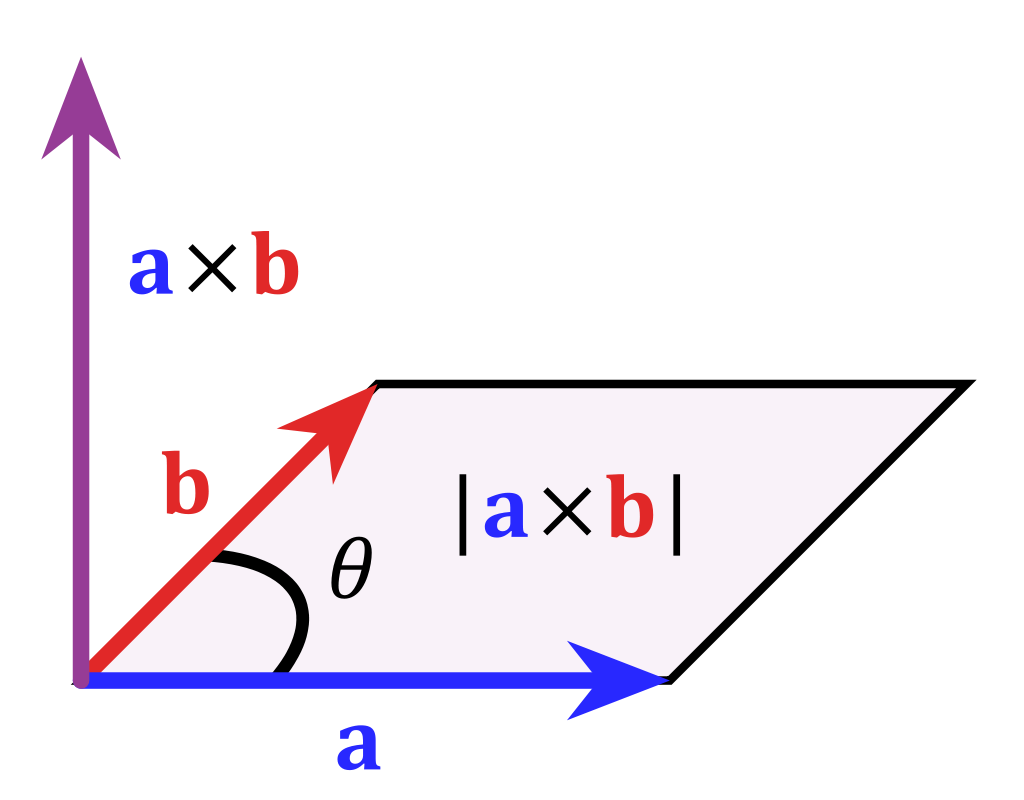
\includegraphics[width=0.4\linewidth]{kreuzprodukt.png}
	\end{figure}
	Dabei berechnen wir das Kreuzprodukt folgender Maßen:
	\Definition{(Kreuzprodukt)}{
		Seien $\vec{a}=\Spvek{a_1;a_2;a_3},\,\vec{b}=\Spvek{b_1;b_2;b_3}\in \mathds{R}^3$\\
		{\large{\[\vec{a} \times \vec{b}= \Spvek{a_2 b_3 - a_3 b_2; a_3 b_1 - a_1 b_3; a_1 b_2 - a_2 b_1}\]}}
	}
	Auch das Kreuzprodukt ist jetzt noch nicht interessant, wird aber auch beim Thema Ebenen wieder benutzt.
	
	\subsection{Geometrische Eigenschaften}
	Im folgenden zähle ich ein paar geometrische Eigenschaften auf, und Wege diese über analytische Geometrie zu verifizieren.
	\begin{itemize}
		\item \textbf{Länge} einer Strecke $\overline{AB}=l$: \[l=\left\vert\, \vec{AB} \,\right \vert\]
		\item \textbf{Rechtwinkligkeit} von 2 Strecken $\overline{AB},\overline{BC}$:
		\[\overline{AB},\overline{BC} \text{ sind rechtwinklig genau dann wenn }\, \vec{AB}\circ \vec{BC}=0\]
		\item \textbf{Parallelität} von zwei Stecken $\overline{AB},\overline{BC}$
			\begin{enumerate}[(i)]
				\item $\overline{AB},\overline{BC}$ sind parallel genau dann wenn
					\[\vec{AB},\vec{BC} \text{ linear abhängig sind}\]
				\item $\overline{AB},\overline{BC}$ sind parallel genau dann wenn
					\[\vec{AB}\circ\vec{BC} = |\vec{AB}|\cdot |\vec{BC}|\quad\text{ oder }\quad\vec{AB}\circ\vec{BC} = -|\vec{AB}|\cdot |\vec{BC}|\]
			\end{enumerate}
	\end{itemize} 
	\Aufgabe{3.8.1 (Vierecke)}{
		Überprüfe ob das Viereck $ABCD$ ein Parallelogramm, eine Raute oder ein Trapez ist.
		Berechne den Flächeninhalt sollte es ein Parallelogramm sein.
		
			\begin{enumerate}[(a)]
				\item $A( 2\,|\,5 \,|\,-2 ),\, B( 5\,|\,2 \,|\, 1),\,C(1 \,|\,-2 \,|\,-1 ),\, D(-2 \,|\,1 \,|\,4 )$
				\item $A( 7\,|\,0 \,|\,6 ),\, B(3 \,|\,-6 \,|\, 4),\,C(7 \,|\,5 \,|\,-2 ),\, D( 5\,|\,2 \,|\, -3)$
				\item $A( 2\,|\,-3 \,|\,-5 ),\, B(0 \,|\, -1\,|\, -2),\,C(4 \,|\,-2 \,|\,-3 ),\, D(-3 \,|\, 4\,|\,3 )$
				\item $A( -3\,|\,2 \,|\,7 ),\, B( 6\,|\,1 \,|\, 3),\,C( 2\,|\,4 \,|\,-3 ),\, D( -7\,|\,5 \,|\,1 )$
				\item $A( 6\,|\,3 \,|\,3 ),\, B(5 \,|\, 5\,|\, -2),\,C( 3\,|\,6 \,|\,3 ),\, D( 4\,|\,4 \,|\,8 )$
			\end{enumerate}
		
	}
	\Aufgabe{3.8.2 (Dreiecke)}{
		Überprüfe ob das Dreieck $ABC$ gleichseitig, gleichschenklig oder rechtwinklig ist.
		Gebe den Umfang und Flächeninhalt an.		
		\begin{enumerate}[(a)]
			\item $A( 3\,|\,7 \,|\,2 ),\, B( -1\,|\,5 \,|\,1 ),\,C(2 \,|\,3 \,|\,0 )$
			\item $A( 0\,|\,3 \,|\,5 ),\, B( 0\,|\,9 \,|\,5 ),\,C(0 \,|\,6 \,|\,8)$
			\item $A( 4\,|\,-1 ),\, B( -2\,|\,-1),\,C( 1\,|\,1)$
			\item $A( -2\,|\,4 \,|\,1 ),\, B( 1\,|\,7 \,|\,4 ),\,C( 0\,|\,6 \,|\,9 )$
			\item $A( 1 \,|\,2 ),\, B( -1\,|\,1),\,C( 2\,|\,-1)$
			\item $A( 1\,|\,0 \,|\,3 ),\, B( 3\,|\,-2 \,|\,0 ),\,C( 2\,|\, -3\,|\,3 )$
			\item $A( -5\,|\, 2\,|\,-1 ),\, B( 0\,|\, 5\,|\,-3 ),\,C(-1 \,|\,6 \,|\, -3)$
			\item $A( 3\,|\,2 ),\, B( 4\,|\,-1),\,C( -1\,|\,1)$
		\end{enumerate}
		
	}
	\newpage
	\section{Geraden}
	Mit unserem neugewonnen Werkzeug den Vektoren können wir jetzt anfangen andere Geometrische Strukturen zu verallgemeinern und in dieser ''Sprache'' formulieren. Geraden wurden von uns, im 2 dimensionalen Fall, bereits in der 8. Klasse beschrieben. Dabei ist die Geradengleichung \[y=\color{red}m\color{black}x+\color{blue}n\color{black}\]
	Daran können wir erkennen was eine Gerade ausmacht:
	\begin{itemize}
		\item Ein Punkt auf der Gerade ($\color{blue}n\color{black}$)
		\item Richtung in die sie verläuft ($\color{red}m\color{black}$)
	\end{itemize}
	Diese beiden Eigenschaften können wir bereits mit Vektoren beschreiben. Wobei der Punk vom Stützvektor beschrieben wird, die Richtung von einer Variable als Skalar und einem Richtungsvektor.
	\Definition{(Gerade)}{
		Eine Gerade $\color{lightblue}g\color{black}$ im $n$-Dimensionalen Raum wird beschrieben durch den Stützvektor $\color{blue}\vec{s}\color{black}\in\mathds{R}^n$ und dem Richtungsvektor $\color{red}\vec{r}\color{black}\in\mathds{R}^n$ sowie einem Skalar als Variable $t$.
		\large
		\begin{align*}
			\color{lightblue}g\color{black}: \,\quad\qquad\vec{x}&=\color{blue}\vec{s}\color{black} + t\cdot\color{red}\vec{r}\color{black} \\\\
			\color{lightblue}g\color{black}: \quad\Spvek{x_1;x_2;\vdots \,\,;x_n}&=\Spvek{s_1;s_2;\vdots \,\,;s_n} + t\cdot \Spvek{r_1;r_2;\vdots \,\,;r_n}
		\end{align*}
	}
	\begin{center}
		\begin{tikzpicture}
			\draw[thin,gray!40] (-1,-1) grid (7,3);
			\draw[<->] (-1,0)--(7,0) node[right]{$x$};
			\draw[<->] (0,-1)--(0,3) node[above]{$y$};
			\draw[line width=2pt,lightblue,dotted](-1,0.33) -- (7,3)node[anchor=north west]{$\vec{g}$};
			\draw[line width=2pt,red,-stealth](1,1) --node[anchor=north west]{$\vec{r}$} (2,1.33);
			\draw[line width=1pt,red,-stealth](1,1) --node[anchor=north west]{$3\cdot \vec{r}$} (4,2);
			\draw[line width=1pt,red,-stealth](1,1) --node[anchor=south east]{$-\frac{3}{2} \vec{r}$} (-0.5,0.5);
			\draw[line width=2pt,blue,-stealth](0,0) --node[anchor=north west]{$\vec{s}$} (1,1);
		\end{tikzpicture}
	\end{center}
	Wie auf dem Bild zu sehen kann je nach wahl von $t$ jeder Punkt auf der Gerade beschrieben werden. Es sollte nun auch klar sein woher die Namen ''Stützvektor'' und ''Richtungsvektor'' kommen.

	\subsection{Konstruktion von Geraden}
	Wie auch schon für $y=mx+n$ können wir solche Geraden anhand von gegebenen Eigenschaften Konstruieren. Solche Eigenschaften können zum Beispiel zwei gegebenen Punkte, welche auf der Gerade liegen sollen, sein. Selterner wird ein Punkt von der Gerade gegeben und ein Richtungsvektor in welche die Gerade verlaufen soll.
	\subsubsection{Gegeben Punkt und Richtung}
	Dies macht uns die konstruktion besonders einfach.
	Sei $P$ der gegebene Punkt, $\vec{r}$ der Richtungsvektor. Die Gerade $g$, welche durch $P$ verläuft mit Richtung $\vec{r}$ wird so konstruiert:
	\Redbox{\large\[g: \,\vec{x} = \overline{0P} + t\cdot \vec{r}\]}
	\subsubsection{Gegeben zwei Punkte}
	Etwas schwieriger wird die Konstruktion mit lediglich 2 gegebenen Punkten.\\
	Sei $A,B$ gegebene Punkte, dann konstruieren wir $g$, indem wir einen der gegebenen Punkte als Stützvektor wählen und für den Richtungsvektor den Vektor, durch den wir von Punkt $A$ zu Punkt $B$ kommen, wählen.
	\Redbox{\large \[g:\, \vec{x}=\overline{0A} +t\cdot \overline{AB} \]}
	\subsection{Lagebeziehung Punkt und Gerade}
	Für einen gegebenen Punkt $P$ und Gerade $g$ kann man entscheiden ob $P$ auf $g$ liegt. Sollte dies nicht der Fall sein ist es weiterhin möglich den Punkt $Q$ auf $g$ anzugeben, welcher am nächsten an $P$ liegt.
	\subsubsection{Liegt der Punkt $P$ auf der Gerade?}
	Gegeben sei Punkt $P=(P_x,P_y,P_z)$ und Gerade $g:\,\, \vec{x}=\Spvek{s_x;s_y;s_z} + t \cdot \Spvek{r_x;r_y;r_z}$.\\
	Um zu überprüfen ob $P$ auf $g$ liegt schaffen wir ein Gleichungssystem:
	\Redbox{\begin{align*}
			\Spvek{P_x;P_y;P_z}&=\Spvek{s_x;s_y;s_z} + t \cdot \Spvek{r_x;r_y;r_z}&&\bigg\vert -\Spvek{s_x;s_y;s_z} \\
			\Spvek{P_x - s_x;P_y-s_y;P_z-s_z} &= t \cdot \Spvek{r_x;r_y;r_z} \qquad \begin{bmatrix}
				t_x=\frac{P_x-s_x}{r_x}\\t_y=\frac{P_y-s_y}{r_y}\\t_z=\frac{P_z-s_z}{r_z}\\
			\end{bmatrix}&&
	\end{align*}}
	Falls nun $t_x=t_y=t_z$ gilt, mit anderen Worten die Lösungsmenge des Gleichungssystems nicht leer ist, dann liegt der Punkt auf der Geraden.\\
	Gilt dies nicht, liegt der Punkt $P$ auch nicht auf der Geraden $g$.
	\subsubsection{Nächste Punkt auf der Geraden}
	\subsection{Lagebeziehungen zwischen Geraden und Geraden}
	Auch kann die Lage zwischen zwei Geraden ermittelt werden, das heißt ob diese sich schneiden, parallel sind, windschief stehen oder aufeinander liegen.\\
	Gegeben Geraden $g:\, \vec{x}_g = \vec{s}_g + t\cdot \vec{r}_g,\quad h:\, \vec{x}_h = \vec{s}_h + k\cdot \vec{r}_h$\\
	Herangehensweise:
	\subsubsection{Auf Schnittpunkt Prüfen}
	Wie bei 2 Geraden der Form $y=mx+n$ müssen wir diese gleichsetzen, also:
	\begin{align*}
		\vec{s}_g + t\cdot \vec{r}_g & = \vec{s}_h + k\cdot \vec{r}_h&&\big \vert -\vec{s}_g,\, -  k\cdot \vec{r}_h\\
		t\cdot \vec{r}_g - k\cdot \vec{r}_h &= \vec{s}_h - \vec{s}_g\\
		t\cdot \Spvek{r_{g_x};r_{g_y};r_{g_z}} - k\cdot \Spvek{r_{h_x};r_{h_y};r_{h_z}} &= \Spvek{s_{h_x}-s_{g_x};s_{h_y}-s_{g_y};s_{h_z}-s_{g_z}}\\
		&\downarrow\\
		r_{g_x}\cdot \color{red}t\color{black} - r_{h_x}\cdot \color{blue}k\color{black} &= s_{h_x}-s_{g_x}\\
		r_{g_y}\cdot \color{red}t\color{black} - r_{h_y}\cdot \color{blue}k\color{black} &= s_{h_y}-s_{g_y}\\
		r_{g_z}\cdot \color{red}t\color{black} - r_{h_z}\cdot \color{blue}k\color{black} &= s_{h_z}-s_{g_z}\\
	\end{align*}
	Dabei sind $\color{blue}k\color{black},\color{red}t\color{black}$ die Variablen. Falls die Lösungsmenge des Gleichungssystems:\begin{enumerate}[(I)]
		\item $|L|=0$ die Geraden schneiden sich nicht
		\item $|L|=1$ die Geraden schneiden sich
		\item $|L|=\infty$ die Geraden liegen aufeinander
	\end{enumerate}
	Für (I) ist nun noch zu prüfen ob die Geraden windschief oder parallel zueinander sind.
	\subsubsection{Auf Lineare Abhängigkeit prüfen}
	Gelte (I), nun ist lediglich die lineare Abhängigkeit zu prüfen, ein Synonym für Parallelität. Setzte die Richtungsvektoren der Geraden mit Hilfe einer Variable  gleich:
	\[\Spvek{r_{h_x};r_{h_y};r_{h_z}} = t \cdot  \Spvek{r_{g_x};r_{g_y};r_{g_z}} \qquad \begin{bmatrix}
		t_x={r_{h_x}}/{r_{g_x}}\\t_y={r_{h_y}}/{r_{g_y}}\\t_z={r_{h_z}}/{r_{g_z}}
	\end{bmatrix}\]
	Falls $t_x=t_y=t_z$ sind die Richtungsvektoren linear abhängig und damit die beiden Geraden parallel.\\ Sonst sind die Geraden windschief.
	\subsection{Aufgaben}
	\Aufgabe{1.4.1: (Konstruktion gegeben 2 Punkte)}{
		\begin{multicols}{2}
			\begin{enumerate}[(a)]
				\item $A=(2\,|\,5\,|\,8),\, B=(1\,|\,2\,|\,9)$
				\item $A=(2\,|\,-5),\, B=(2\,|\,10)$
				\item $A=(-12\,|\,2,5\,|\,3),\, B=(5\,|\,-4,5\,|\,7)$
				\item $A=(0\,|\,0\,|\,-10),\, B=(10\,|\,-6\,|\,4)$
				\item $A=(4\,|\,4\,|\,3),\, B=(4\,|\,4\,|\,3)$
				\item $A=(2\,|\,-5\,|\,2),\, B=(8\,|\,7\,|\,-4)$
			\end{enumerate}
		\end{multicols}
	}
	\Aufgabe{1.4.2: (Lagebeziehung Punkt - Gerade)}{
		\begin{multicols}{2}
			\begin{enumerate}[(a)]
				\item $g:\, \vec{x}=\Spvek{3;2;-3}+ t\cdot \Spvek{1;0;1}$\\\\
				$P=(3\,|\,4\,|\,-1)$
				\item $g:\, \vec{x}=\Spvek{3;2;-3}+ t\cdot \Spvek{1;0;1}$\\\\
				$P=(6\,|\,2\,|\,0)$
				\item $g:\, \vec{x}=\Spvek{3;2;-3}+ t\cdot \Spvek{1;0;1}$\\\\
				$P=(-5\,|\,2\,|\,-10)$
				\item $g:\, \vec{x}=\Spvek{1;-1;0}+ t\cdot \Spvek{-1;0;-3}$\\\\
				$P=(2\,|\,-1\,|\,9)$
				\item $g:\, \vec{x}=\Spvek{1;-1;0}+ t\cdot \Spvek{-1;0;-3}$\\\\
				$P=(0\,|\,2\,|\,-3)$
				\item $g:\, \vec{x}=\Spvek{1;-1;0}+ t\cdot \Spvek{-1;0;-3}$\\\\
				$P=(2\,|\,-1\,|\,3)$
			\end{enumerate}
		\end{multicols}
	}
	\Aufgabe{1.4.3: (Lagebeziehung Gerade - Gerade)}{
		\begin{multicols}{2}
			\begin{enumerate}[(a)]
				\item $g:\, \vec{x}=\Spvek{3;2;-3}+ t\cdot \Spvek{1;0;1}$\\\\\\
						$h:\, \vec{x}=\Spvek{3;2;-3}+ k\cdot \Spvek{1;0;1}$
				\item $g:\, \vec{x}=\Spvek{3;2;-3}+ t\cdot \Spvek{1;0;1}$\\\\\\
				$h:\, \vec{x}=\Spvek{3;2;-3}+ k\cdot \Spvek{1;0;1}$ 
				\item $g:\, \vec{x}=\Spvek{3;2;-3}+ t\cdot \Spvek{1;0;1}$\\\\\\
				$h:\, \vec{x}=\Spvek{3;2;-3}+ k\cdot \Spvek{1;0;1}$
				\item $g:\, \vec{x}=\Spvek{3;2;-3}+ t\cdot \Spvek{1;0;1}$\\\\\\
				$h:\, \vec{x}=\Spvek{3;2;-3}+ k\cdot \Spvek{1;0;1}$
				\item $g:\, \vec{x}=\Spvek{3;2;-3}+ t\cdot \Spvek{1;0;1}$\\\\\\
				$h:\, \vec{x}=\Spvek{3;2;-3}+ k\cdot \Spvek{1;0;1}$
				\item $g:\, \vec{x}=\Spvek{3;2;-3}+ t\cdot \Spvek{1;0;1}$\\\\\\
				$h:\, \vec{x}=\Spvek{3;2;-3}+ k\cdot \Spvek{1;0;1}$
			\end{enumerate}
		\end{multicols}
	}
	%\section{Ebenen}
	
\end{document} 